\chapter{Diseño Analítico}

A partir de las especificaciones de diseño de la Tabla \ref{tab:specs}, una vez ingresados en el software de diseño de filtros se obtuvo que este tendrá las características detalladas en la Tabla \ref{tab:frecuencias} y deberá cumplir con la plantilla en \ref{fig:plantilla}.

\begin{table}[ht]
\begin{center}
\begin{tabular}{||c|c||}
\hline
Ganancia	&	$0.5 \si{\deci\bel}$	\\
\hline	
$f_a^-$		&	$615 \si{\hertz}$	\\
\hline	
$f_p^-$		&	$2.07 \si{\kilo\hertz}$	\\
\hline	
$f_p^+$	&	$12.07 \si{\kilo\hertz}$	\\
\hline	
$f_a^+$	&	$40.62 \si{\kilo\hertz}$	\\
\hline	
$A_a$		&	$50 \si{\deci\bel}$	\\
\hline	
$A_p$		&	$0.5 \si{\deci\bel}$	\\
\hline	
Orden		&	$4$	\\
\hline	
\end{tabular}
\caption{Características del filtro pasa bandas diseñado}
\label{tab:frecuencias}
\end{center}
\end{table}

\begin{figure}[ht]
\begin{center}
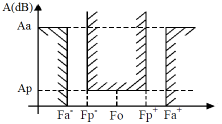
\includegraphics{../Diseño/publish/Plantillas/BandpassImg2.png}
\caption{Plantilla del Filtro Pasa Bajos}
\label{fig:plantilla}
\end{center}
\end{figure}

Habiendo ingresado las especificaciones del filtro al software de diseño de filtros y de separación de etapas, el filtro fue finalmente implementado utilizando dos etapas pasa altos de segundo orden y dos etapas pasa bajos de segundo orden en cascada.

\begin{figure}[ht]
\begin{center}
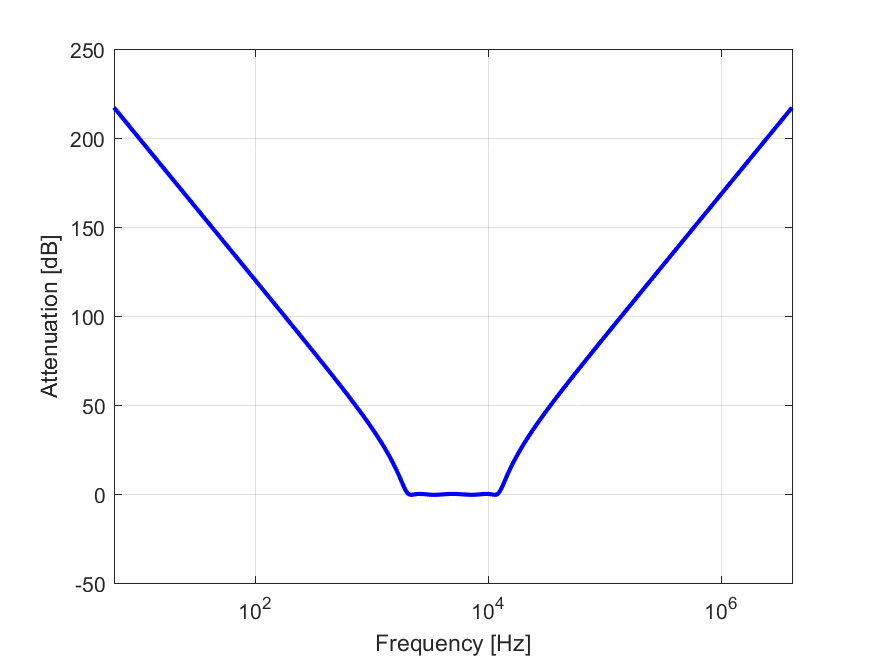
\includegraphics[width=0.45 \linewidth]{../Diseño/publish/Filter_Atte.png}
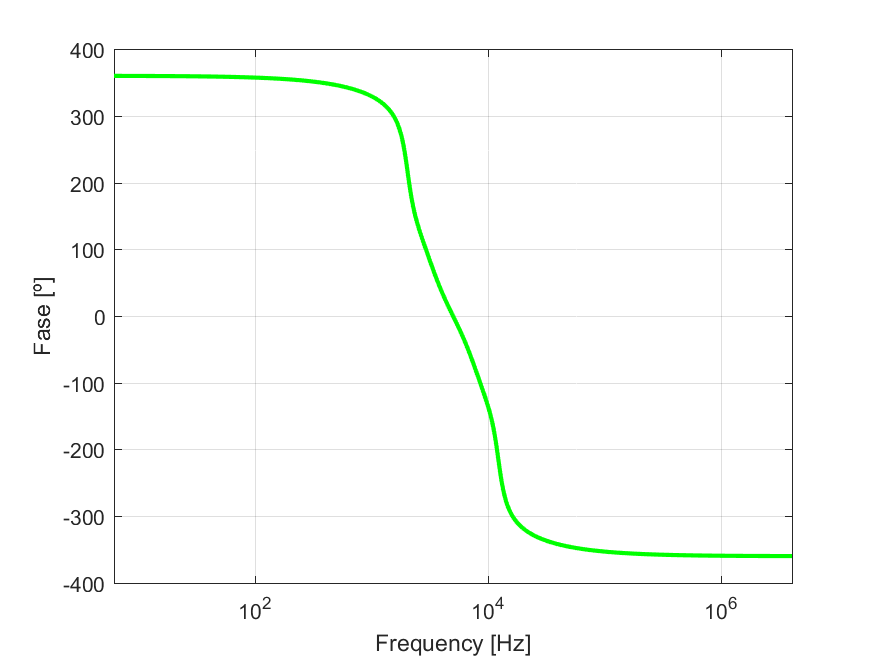
\includegraphics[width=0.45 \linewidth]{../Diseño/publish/Filter_Phase.png}
\caption{Transferencia del filtro completo}
\end{center}
\end{figure}

\begin{figure}[ht]
\begin{center}
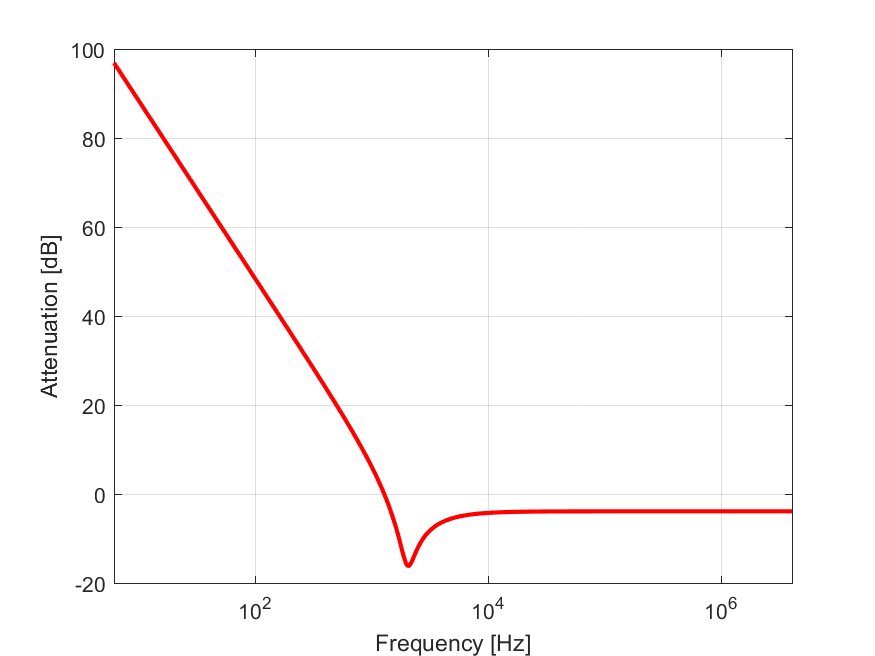
\includegraphics[width=0.45 \linewidth]{../Diseño/publish/Stage1_Att.png}
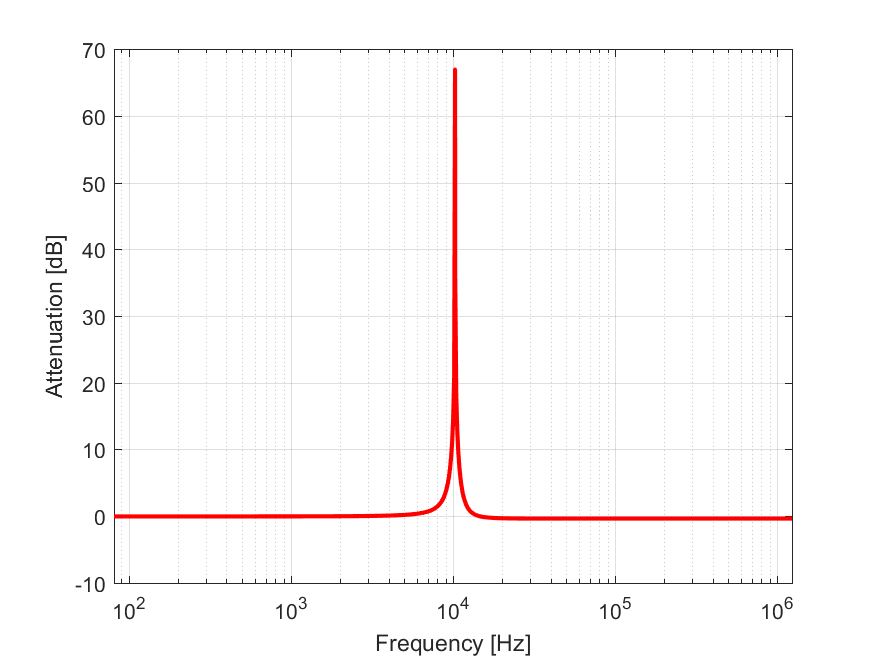
\includegraphics[width=0.45 \linewidth]{../Diseño/publish/Stage2_Att.png}
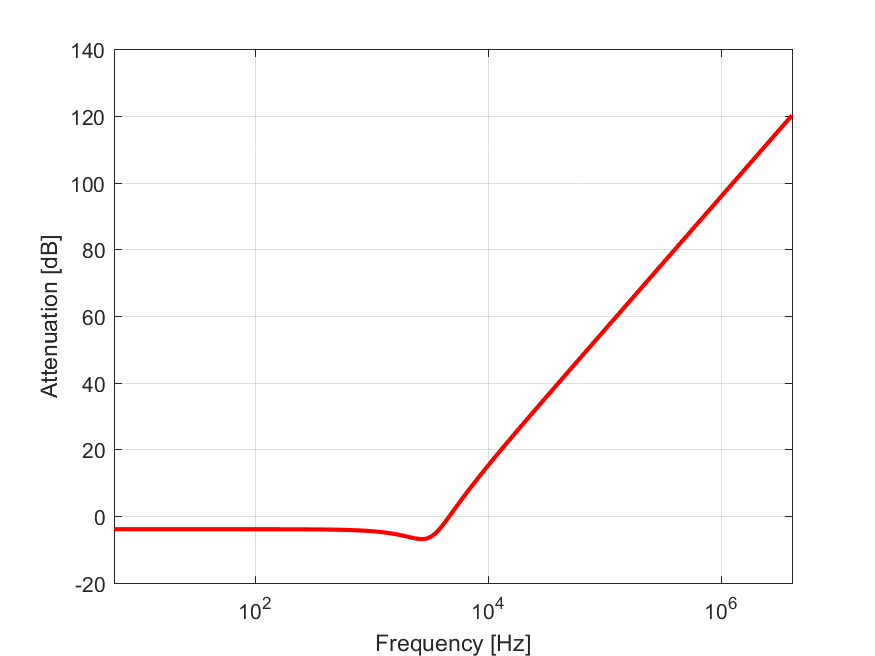
\includegraphics[width=0.45 \linewidth]{../Diseño/publish/Stage3_Att.png}
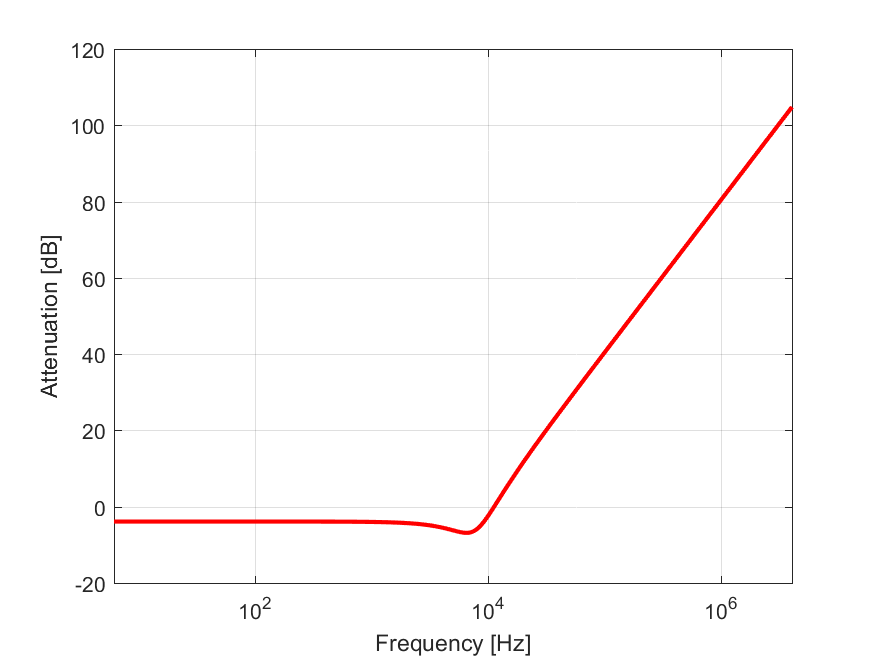
\includegraphics[width=0.45 \linewidth]{../Diseño/publish/Stage4_Att.png}
\caption{Atenuación las cuatro etapas}
\end{center}
\end{figure}